% Chapter Template

\chapter{Theory} % Main chapter title

\label{Chapter2} % Change X to a consecutive number; for referencing this chapter elsewhere, use \ref{ChapterX}

\lhead{Chapter 2. \emph{Theory}} % Change X to a consecutive number; this is for the header on each page - perhaps a shortened title

%----------------------------------------------------------------------------------------
%	SECTION 1
%----------------------------------------------------------------------------------------

\section{Cavity Flame-holding}




%----------------------------------------------------------------------------------------
%	SECTION 2
%----------------------------------------------------------------------------------------

\section{Cavity Acoustics}





%------------------------------------------------------------------
%    FIGURES
%-----------------------------------------------------------------


\begin{figure}
\centering
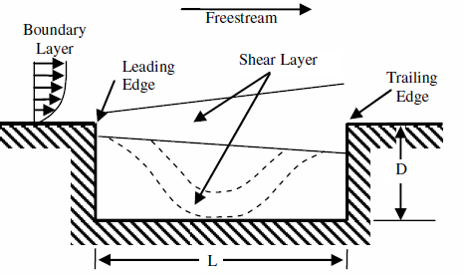
\includegraphics[height=3in]{Figures/CavityDiagram.png}
\caption[Diagram of typical cavity]{Typical hypersonic cavity schematic \cite{lazar2008control}.}
\end{figure}